\documentclass[12pt]{article}

% Packages for basic formatting
\usepackage{amsmath}  % for mathematical symbols
\usepackage{amsfonts} % for fonts
\usepackage{amssymb}  % for more symbols
\usepackage{geometry} % to customize page layout
\usepackage{fancyhdr} % for custom headers
\usepackage{hyperref} % for clickable references
\usepackage{tikz}     % optional, for drawings
\usepackage{graphicx} % optional, for images


\usepackage{listings}
\usepackage{xcolor}
\usepackage{bold-extra}
\usepackage[shortlabels]{enumitem}
\usepackage{tabularx}
\usepackage{gospel}
\usepackage{caption}

\setlist[enumerate]{font=\bfseries}
\DeclareCaptionFormat{listing}{\hfill#3}
\captionsetup[lstlisting]{format=listing,singlelinecheck=false, margin=0pt,
  font={sf,it},labelsep=space,labelfont=bf,belowskip=-1pt}
\captionsetup{justification=centering, labelformat=simple}

% Page dimensions and margins
\geometry{top=1in, bottom=1in, left=1in, right=1in}

% Title info
\title{\textbf{Python Journey} \\ \large Introductory Problem Set}
\date{\today}

\begin{document}

% Title
\maketitle

% Instructions (if any)
\noindent \textbf{Disclaimer} \\\\
In this handout we assume that students:
\begin{itemize}
    \item Have already been introduced to Python functions, conditionals, 
      for and while loops.
    \item Program through scripts instead of using the console.
    \item The objective of these exercises is to reach a simple and intuitive
      solution, which not always corresponds to the most efficient or complete.
\end{itemize}

\subsection*{Exercise 1 - Even Odd} 
\begin{enumerate}[a)]
  \item Develop a function that receives an integer and calculates whether it 
    is odd or even.
  \item Develop a test function for the Even Odd problem.
\end{enumerate}

\subsection*{Exercise 2 - Grade Calculator} 

The following grading system is commonly used in the United States of America:
\begin{table}[!ht]
  \begin{center}
      \begin{tabular}{ | m{7em} | m{7em} | }
          \hline
          Letter Grade  & Number Grade    \\
          \hline
          A             & 90-100          \\
          \hline
          B             & 80-89           \\
          \hline
          C             & 70-79           \\
          \hline
          D             & 60-69           \\
          \hline
          F             & 0-59             \\
          \hline
      \end{tabular}
  \end{center}
\end{table}
\vspace{-1cm}
\begin{enumerate}[a)]
  \item Develop a function that receives an integer and calculates the 
    corresponding letter grade. \textbf{Remember} to verify if the number 
    received is within the desired scale.
  \item Develop a test function for the Grade Calculator problem.
\end{enumerate}

\subsection*{Exercise 3 - List Summation}

Let $a = a_{0}, ..., a_{n-1}$, then $a$ is sequence with $n$ elements, starting from
index $0$ to $n-1$. The sum of the elements in sequence $a$, can be expressed as: 

\[ \sum_{i=0}^{n-1} a_{i} = a_{0} + ... + a_{n-1} \]

\vspace{2mm}
\noindent \textbf{Note} that sequences can be stored as lists in python.
\begin{enumerate}[a)]
  \item Develop a function that receives a list of floats and calculates the
    sum of its elements.
  \item Develop a test function for the List Summation problem.
  \item \textbf{Challenge:} Repeat the previous subproblems, but only sum the 
    even numbers in the list.
\end{enumerate}

\subsection*{Exercise 4 - Vowel Count}
\begin{enumerate}[a)]
  \item Develop a function that calculates the number of vowels in a string. \\
    \textbf{Warning}: The comparison between strings is \textbf{case-sensitive}.
  \item Develop a test function for the Vowel Count problem.
\end{enumerate}

\subsection*{Exercise 5 - Multiplication Table}
Multiplication tables are often used when teaching students multiplication for
the first time, one example being:

\begin{table}[!ht]
  \begin{center}
      \begin{tabular}{ | m{7em} | }
          \hline
          Tabuada do 2  \\
          \hline
          $2 * 1 = 2$   \\
          \hline
          $2 * 2 = 4$   \\
          \hline
          $2 * 3 = 6$   \\
          \hline
          $2 * 4 = 8$   \\
          \hline
          $2 * 5 = 10$  \\
          \hline
          $2 * 6 = 12$  \\
          \hline
          $2 * 7 = 14$  \\
          \hline
          $2 * 8 = 16$  \\
          \hline
          $2 * 9 = 18$  \\
          \hline
          $2 * 10 = 20$ \\
          \hline
      \end{tabular}
  \end{center}
\end{table}

\begin{enumerate}[a)]
  \item Develop an interactive program that prints the multiplication table
    for numbers selected by the user one at a time. The user should also be
    able to terminate the program, for instance with the word "end". 
    \textbf{Remember} to verify if the input is valid.
\end{enumerate}

\subsection*{Exercise 6 - Palindromes}
A palindrome is a sequence of symbols that can be read forward and backwards
in the same way. However, one may usually find that some liberties are taken,
for instance with punctuation or formatting. For simplicity, we recommend
only considering truly palindromic sequences of characters, i.e. the characters
must exactly match in both ways, with the only exception being the letter cases, 
if the student wishes. \\

\noindent By our definition:
\noindent \begin{itemize}
  \item "Stop pots" is truly palindromic, if one ignores letter cases;
  \item "Never odd or even" is not truly palindromic, since the 5th character 
    from the start is "r" and from the back is a space.
\end{itemize}

\begin{enumerate}[a)]
  \item Develop a function that determines whether a string is truly palindromic.
  \item Develop a test function for the Palindromes problem.
\end{enumerate}

\subsection*{Exercise 7 - Fibonacci}
There are innumerous ways to calculate the $n^{th}$ number in the Fibonacci 
sequence. However, in this exercise students should use the iterative method, 
which means starting from the first and second Fibonacci numbers until one
reaches the $n^{th}$ number, using a loop.
\begin{enumerate}[a)]
  \item Develop a function that calculates the $n^{th}$ Fibonacci number.
  \item Develop a test function for the Fibonacci problem.
\end{enumerate}

\subsection*{Exercise 8 - Maximum Element}
\begin{enumerate}[a)]
  \item Develop a function that calculates the maximum element of a list of 
    floats. \\ \textbf{Suggestion:} The resolve variable can be initialized as 
    $float(inf)$
  \item Develop a test function for the Maximum problem.
  \item Repeat the previous subproblems for the minimum element.
  \item \textbf{Challenge:} Repeat the previous subproblems for the second-highest
    value of a list.
\end{enumerate}

\subsection*{Exercise 9 - Prime Numbers}
A prime number is any integer greater than one and only be divisible by itself 
and one. The first five prime numbers are: $2, 3, 5, 7, 11$.

\begin{enumerate}[a)]
  \item Develop a function that calculates if a given integer is a prime number.
  \item Develop a test function for the Prime Numbers problem.
\end{enumerate}

\subsection*{Exercise 10 - Inversion}
\begin{enumerate}[a)]
  \item Develop a function that inverts the order of the elements in a list. 
    \textbf{Suggestion:} The result should be a new list.
  \item Develop a test function for the Inversion problem.
\end{enumerate}

\subsection*{Exercise 11 - Remove Duplicates}
\begin{enumerate}[a)]
  \item Develop a function that removes the elements that are duplicated in a 
  list. \textbf{Suggestion:} The result should be a new list.
  \item Develop a test function for the Remove Duplicates problem.
\end{enumerate}

\subsection*{Exercise 12 - Digit Sum}
\begin{enumerate}[a)]
  \item Develop a function that calculates the sum of all digits of an integer. 
  \textbf{Suggestion:} Convert the integer to a string and only consider 
    non-negative values.
  \item Develop a test function for the Digit Sum problem.
\end{enumerate}

\subsection*{Exercise 13 - Digital Root}
The digital root of a number is the repeated sum of digits until the result only
contains a single digit. For instance:
\[\text{Digit sum of } 9045 = 18 \text{, because } 9+0+4+5 = 18\]
\[\text{Digital root of } 9045 = 9 \text{, because } 9+0+4+5 = 18 \text{ and } 
1+8 = 9 \]
\begin{enumerate}[a)]
  \item Develop a function that calculates the digital root of an integer. 
  \textbf{Suggestion:} Use the function from the previous exercise until the 
    stopping condition is met.
  \item Develop a test function for the Digit Root problem.
\end{enumerate}

\subsection*{Exercise 14 - Count Character}
\begin{enumerate}[a)]
  \item Develop a function that calculates the number of times a character
    occurs in a string. \textbf{Warning:} Remember that python does not support 
    characters directly like other languages, as such, one must use a string and 
    guarantee that it has length of one.
  \item Develop a test function for the Count Character problem.
\end{enumerate}

\subsection*{Exercise 15 - Factorial}
Similar to the Fibonacci sequence, there are various ways to calculate the
factorial of a number, and once more, the objective will be to use its iterative
version. However, in this case, one may iterate over the loop forward or 
backwards.
\begin{enumerate}[a)]
  \item Develop a function that calculates the factorial of a number $n$ by 
    looping forward, i.e., from $1$ to $n$.
  \item Develop a function that calculates the factorial of a number $n$ by 
    looping backwards, i.e., from $n$ to $1$.
  \item Develop a test function for the Factorial problem.
\end{enumerate}

\subsection*{Exercise 16 - Common Elements}
\begin{enumerate}[a)]
  \item Develop a function that calculates the number of common elements at the 
    \textbf{same position} of two lists. \textbf{Warning:} the two lists may be 
    of different sizes, as such, beware of indexes out of bound.
  \item Develop a test function for the Common Elements problem.
\end{enumerate}

\subsection*{Exercise 17 - Remove Element}
\begin{enumerate}[a)]
  \item Develop a function that removes a given element from a list. 
    \textbf{Warning:} The element may be repeated multiple times in the list.
    \textbf{Suggestion:} The result should be in a new list.
  \item Develop a test function for the Common Elements problem.
\end{enumerate}

\subsection*{Exercise 18 - Linear Search}
Linear Search is the most intuitive and simple searching algorithm. It consists
in going from position to position in a list and checking whether the element
stored there is the desired element. The algorithm returns a boolean to indicate
whether it was found.
\begin{enumerate}[a)]
  \item Develop a function that implements linear search.
  \item Develop a test function for the Linear Search problem.
\end{enumerate}

\subsection*{Exercise 19 - Sorted}
\begin{enumerate}[a)]
  \item Develop a function to check if a list is sorted \textbf{ascendingly}.
  \item Develop a test function for the Sorted problem.
\end{enumerate}

\subsection*{Exercise 20 - Binary Search}
Imagine that we have a sorted list, and we are looking for a specific value,
would linear search be efficient? Possibly not, we might be looking for large
value present at the end of a very large list. A common and efficient solution 
used in various fields of Engineering is to divide the domain in half, and if
possible exclude one of the two halves. Binary Search does exactly that, since
the list must be sorted beforehand, by checking the value at the middle point,
we can restrict the domain in half in case the middle point is not the value
we are looking for. This process can be repeated until the domain is valid.
For clarity, see the following Images:

\begin{figure}[h]
  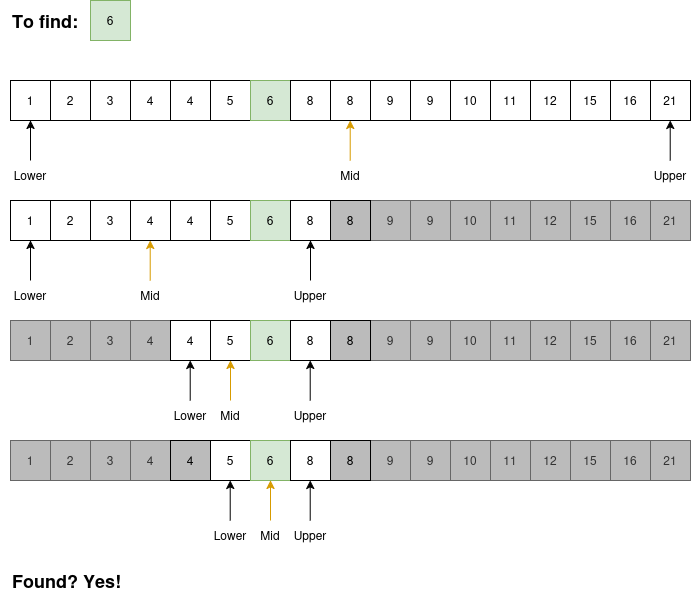
\includegraphics[width=0.5\textwidth]{../Images/BinarySearchFound.png}
  \centering
\end{figure}
\hfill
\begin{figure}[h]
  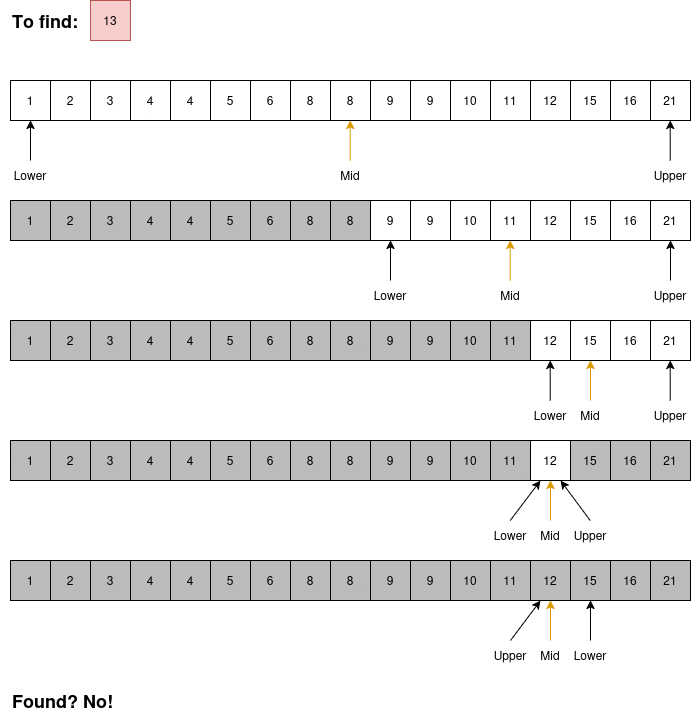
\includegraphics[width=0.5\textwidth]{../Images/BinarySearchNotFound.png}
  \centering
\end{figure}
\vspace{1cm}
\begin{enumerate}[a)]
  \item Complete the following function:
    \begin{pythonlst}
def bin_search(l:list[int], n: int) -> bool:
  assert is_sorted(l)

  lower = #TODO
  upper = #TODO

  while lower <= upper:
    mid = #TODO
    if l[mid] == n:
      return #TODO
    elif l[mid] > n:
      upper = mid - 1
    else:
      lower = mid + 1

  return #TODO
    \end{pythonlst}
  \item Develop a test function for the Binary Search problem.
\end{enumerate}

\end{document}